\begin{figure}
\centering
\subfloat[\sffamily\label{fig:fractionabundancescellcount}]{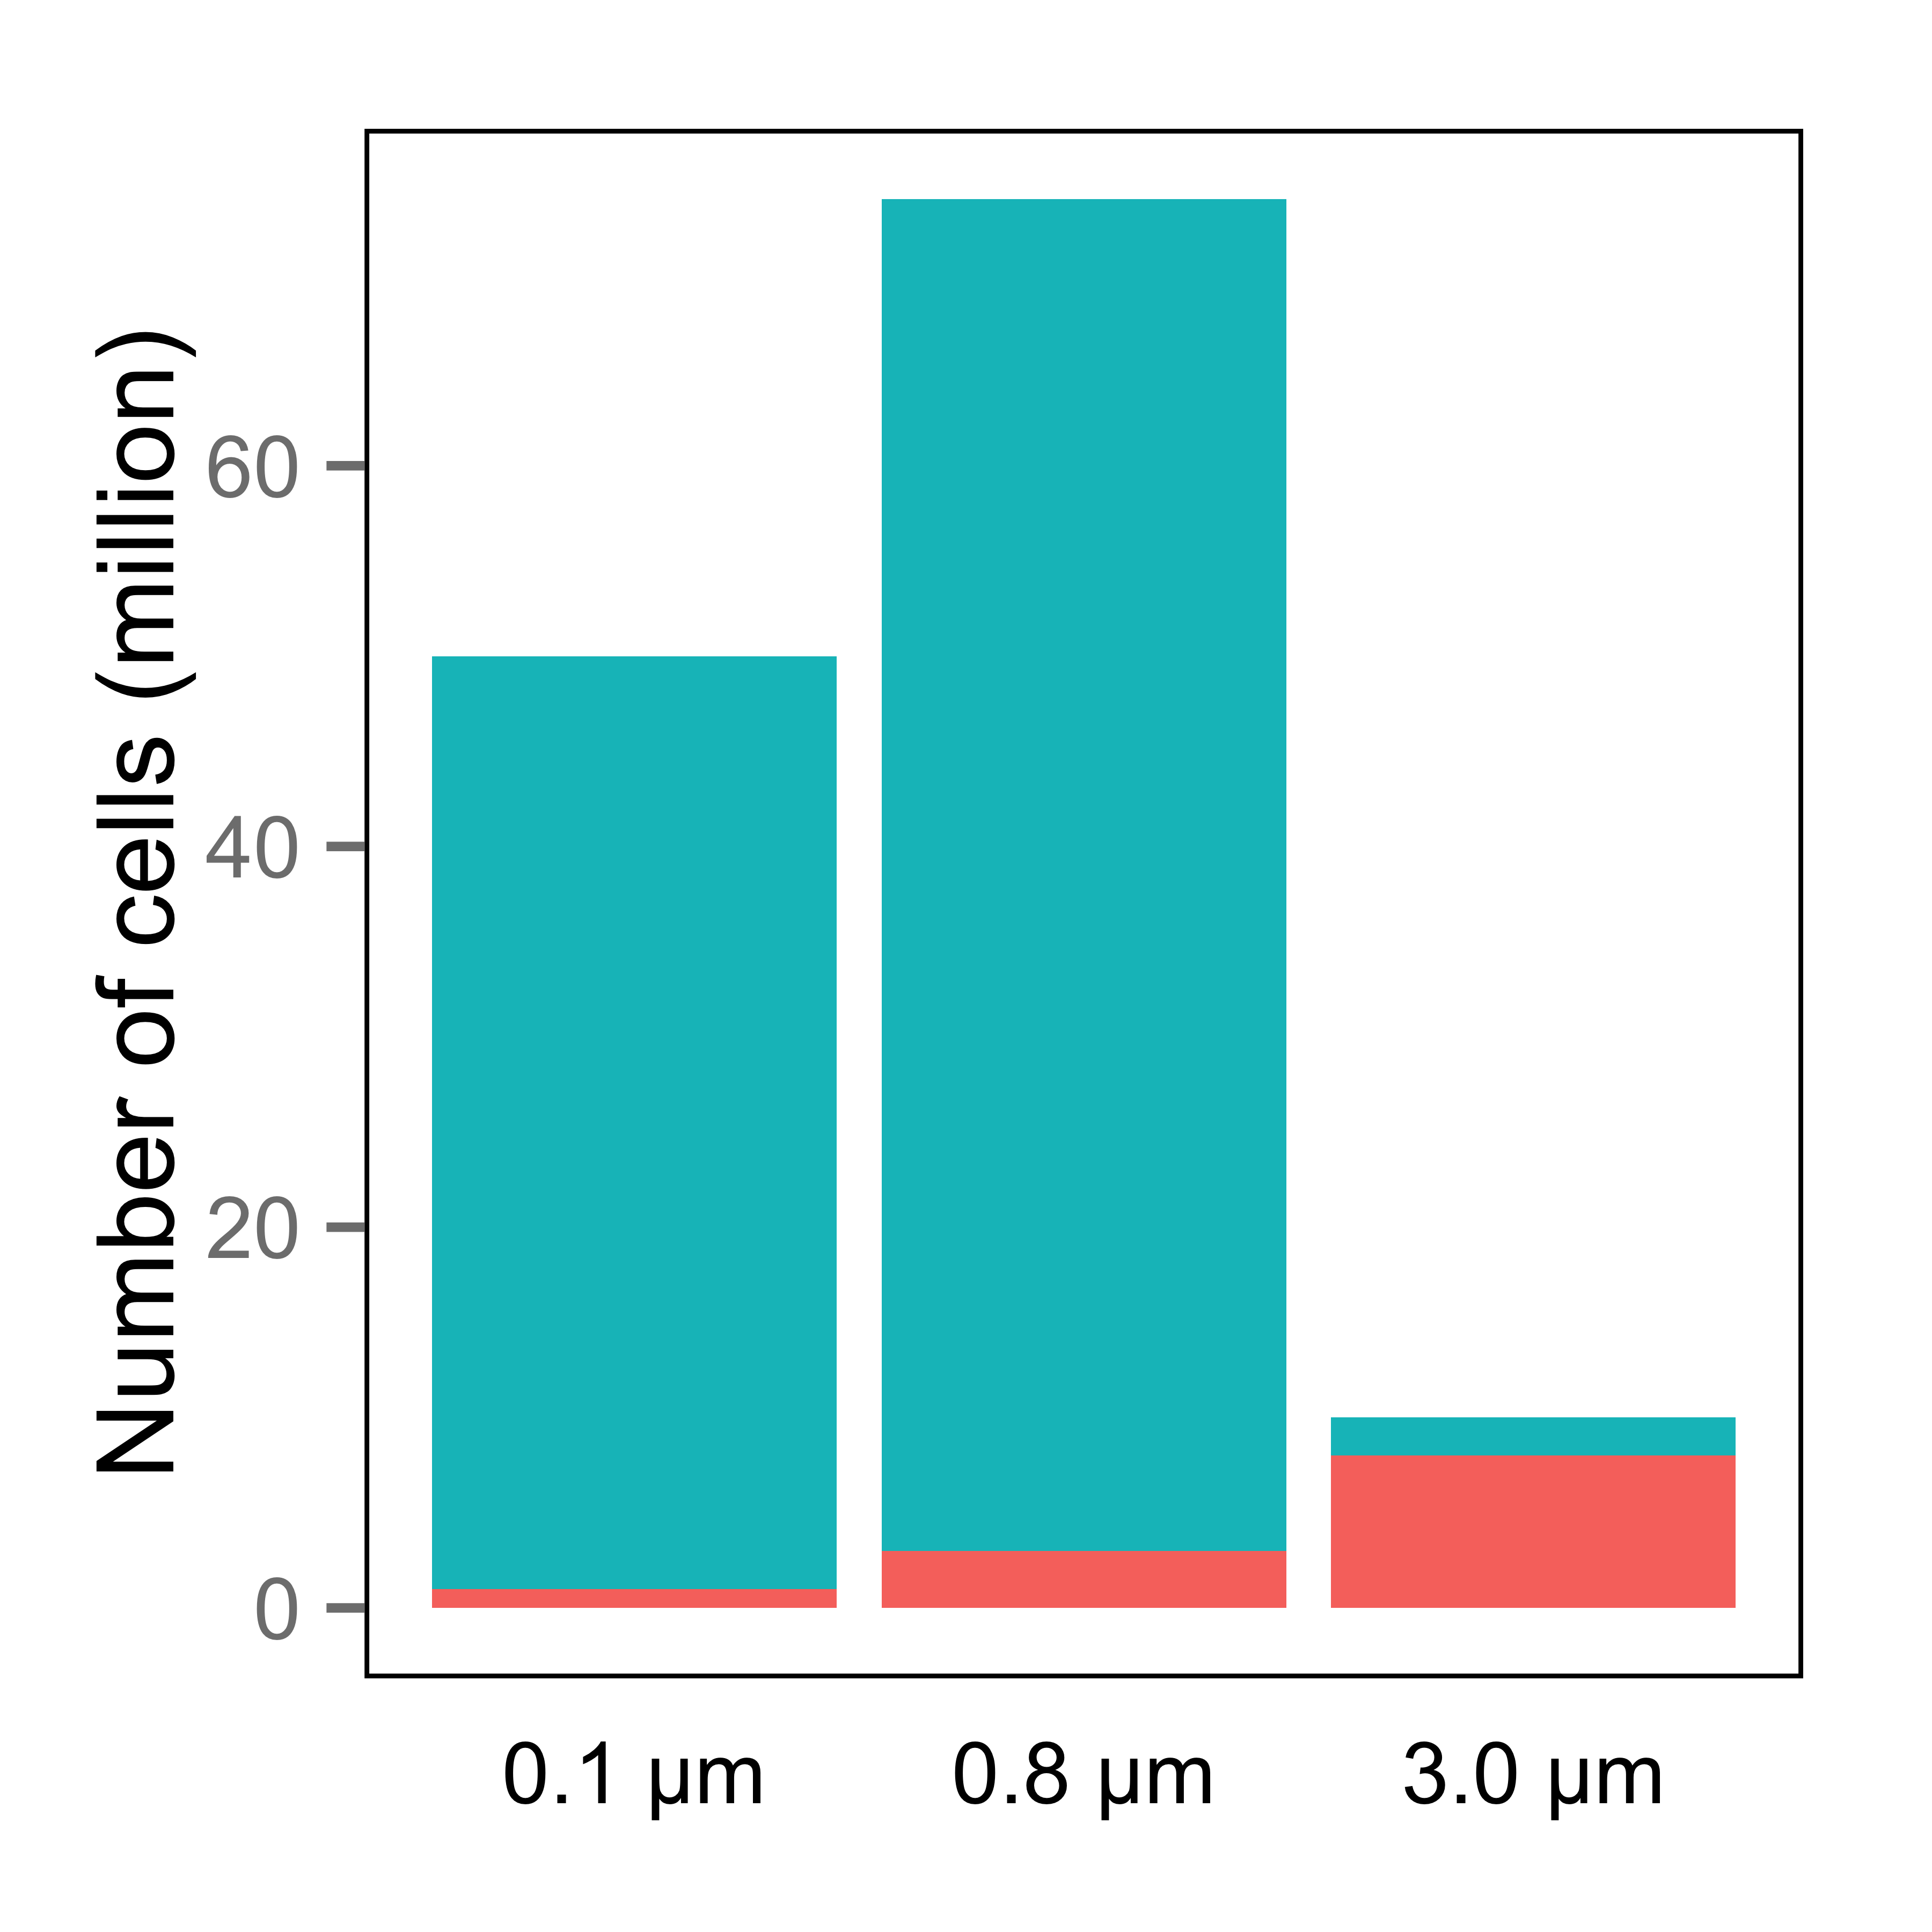
\includegraphics[scale=0.04]{../polarfront/fractionabundances1.png}}
\quad
\subfloat[\sffamily\label{fig:fractionabundancesrelative}]{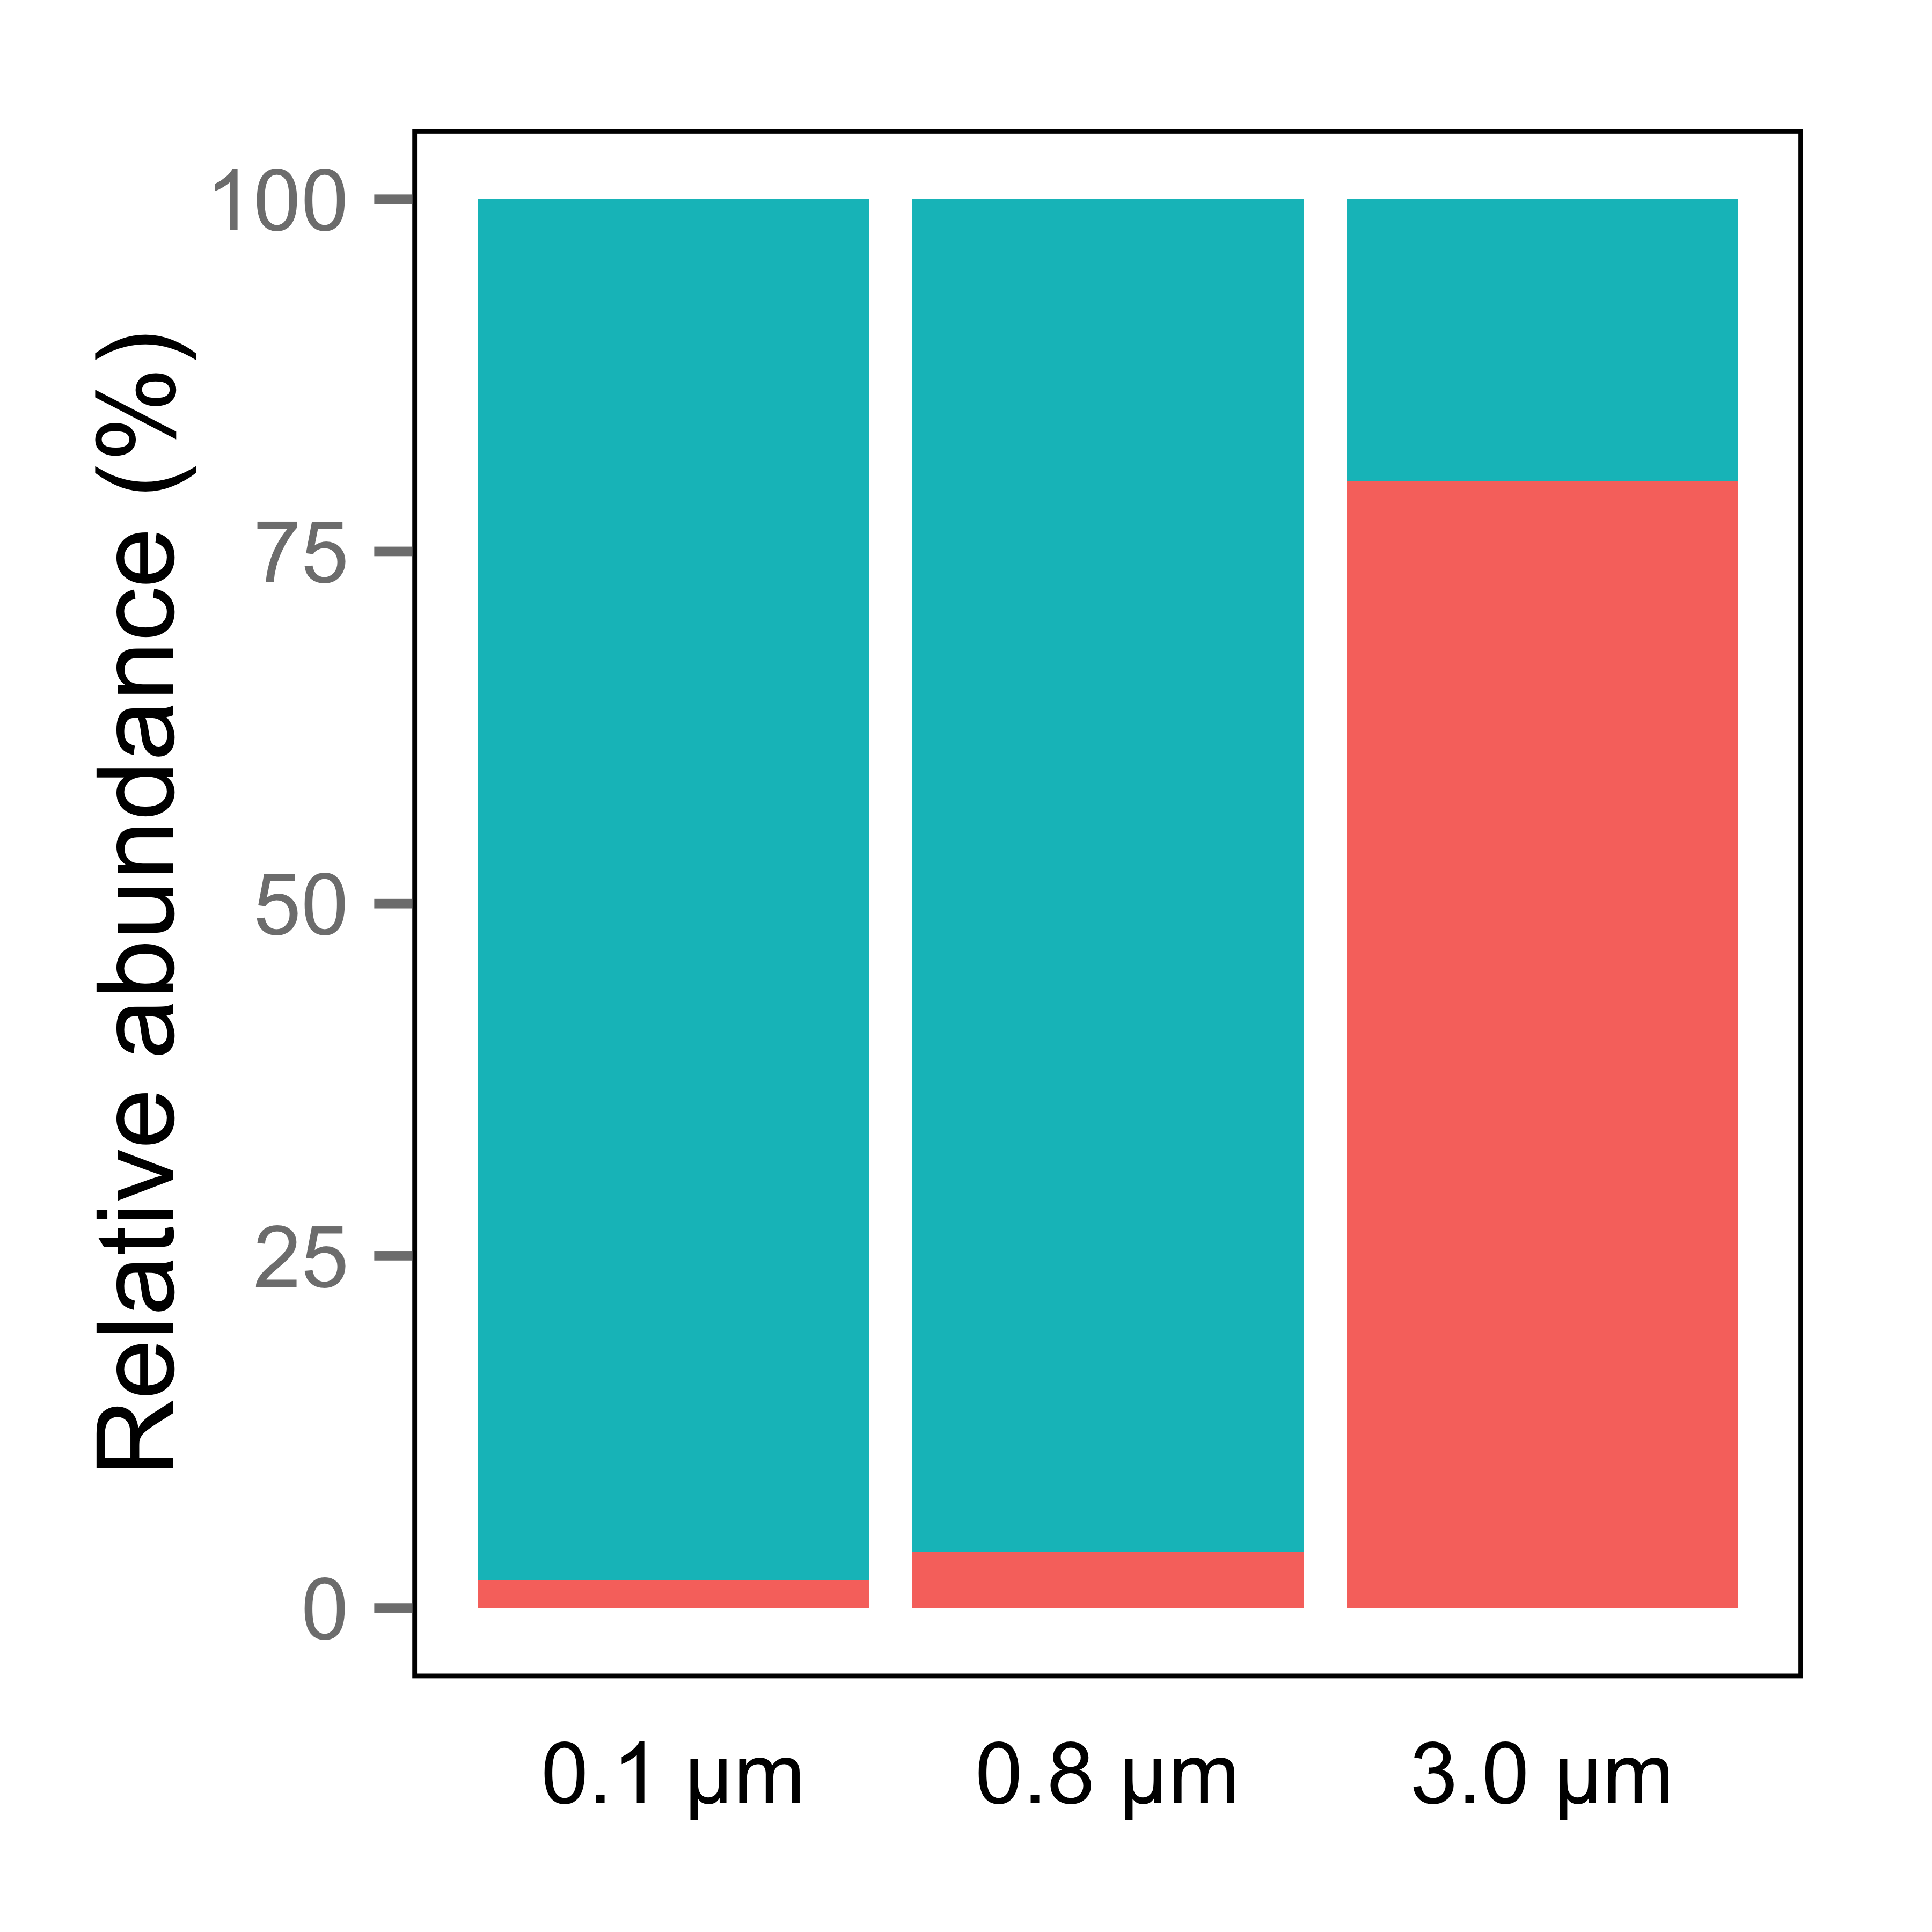
\includegraphics[scale=0.04]{../polarfront/fractionabundances2.png}}
\quad
\subfloat[\sffamily\label{fig:fractionabundancescombined}]{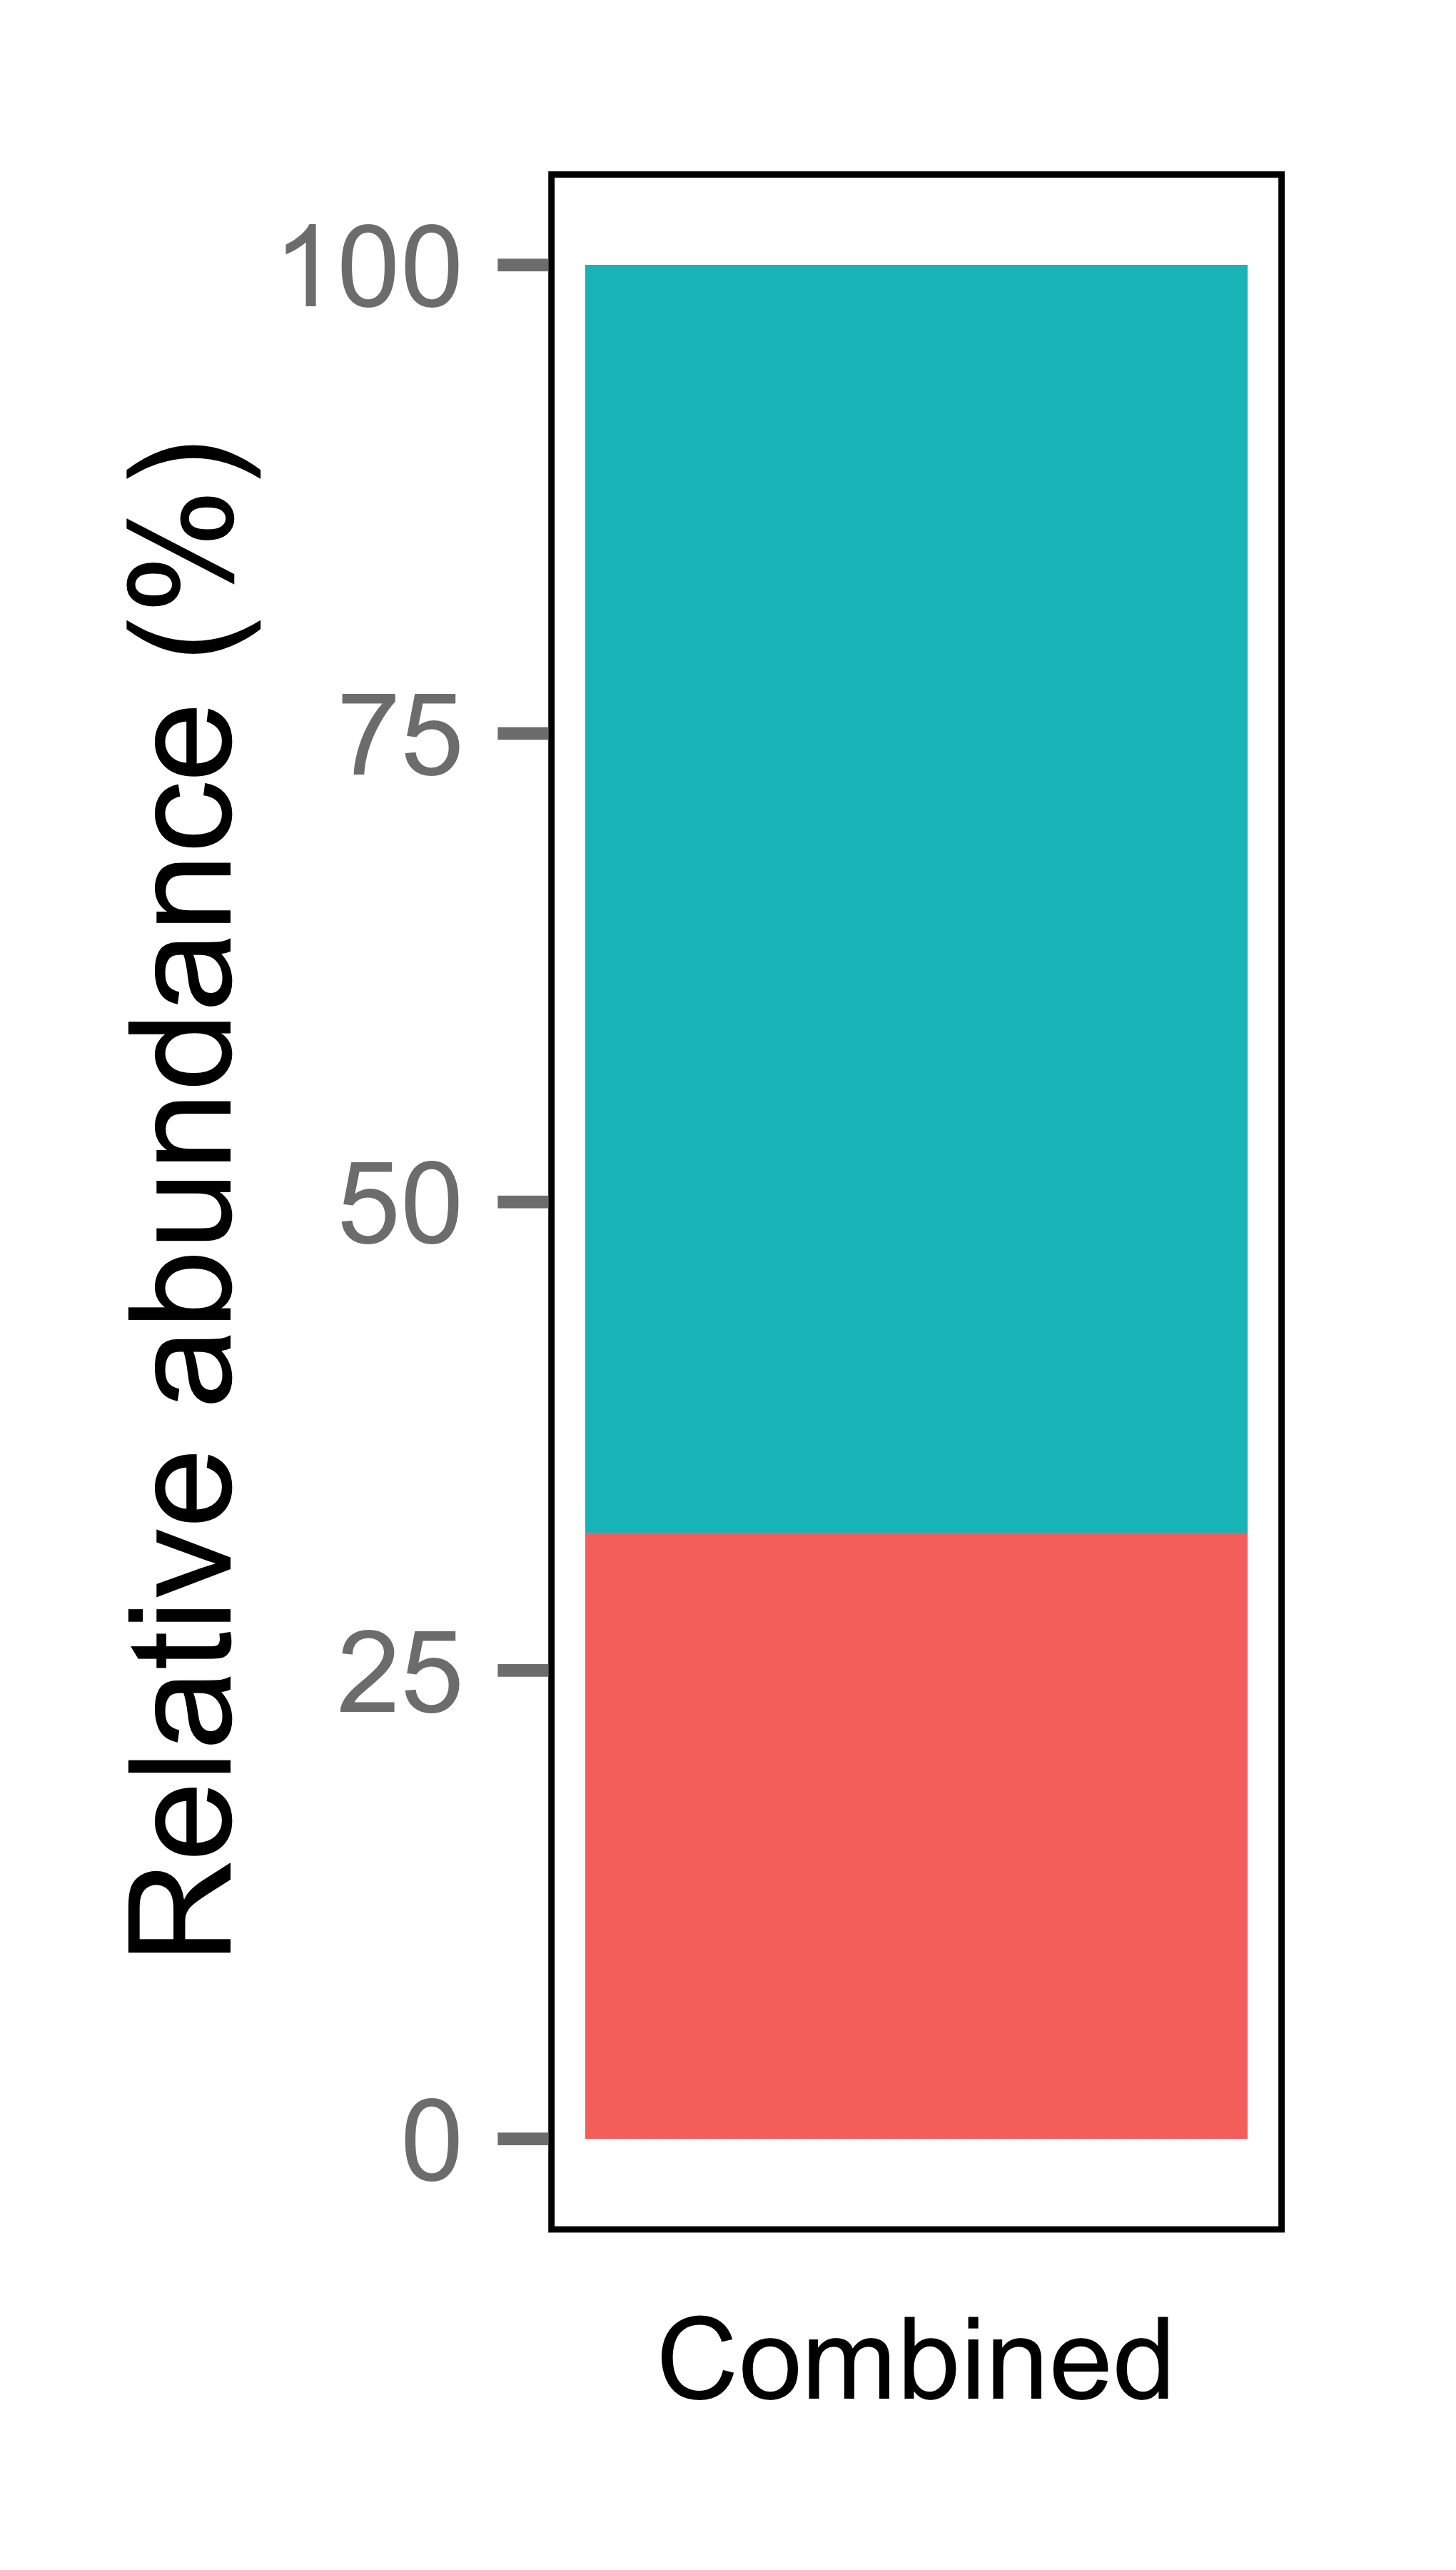
\includegraphics[scale=0.04]{../polarfront/fractionabundances3.png}}
\caption[Summing relative abundances across size fractions]{A visual demonstration of the error introduced by summing OTU relative abundances across size fractions. The red OTU composes only 15\% of the \emph{absolute} number of cells captured (a). However, it has a high \emph{relative} abundance (80\%) in the 3.0 \micron{} fraction (b). A metagenomic analysis without cell counts for each size fraction is only able to determine these relative abundances. If the relative abundances for each fraction are simply summed, the red OTU appears to compose 32\% of the community, more than twice the correct value (c). Without cell counts for each fraction, relative abundances cannot be summed between the fractions.}
\label{fig:fractionabundances}
\end{figure}
